Lempel-Ziv-Welch (LZW) is a widely known lossless, dictionary-based compression algorithm that builds upon the pioneering work of Abraham Lempel and Jacob Ziv on LZ78, published in 1978 in \textit{IEEE Transactions on Information Theory}\cite{doc1}. Terry Welch further refined the algorithm to improve its efficiency and adaptiveness, leading to his 1984 article, "A Technique for High-Performance Data Compression"\cite{doc2}, published in \textit{Computer}.

% \begin{figure}[htbp]
%     \centering
%     % 1st Image
%     \begin{subfigure}[b]{0.4\textwidth}
%         \centering
%         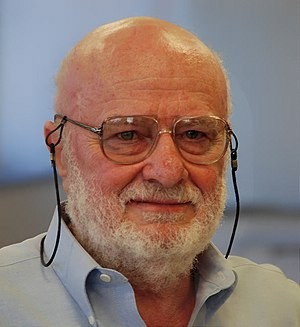
\includegraphics[width=\textwidth]{Figures/lempel.jpg}
%         \caption{Abraham Lempel}
%         \label{fig:lempel}
%     \end{subfigure}
%     \hfill
    
%     % 2nd image
%     \begin{subfigure}[b]{0.4\textwidth}
%         \centering
%         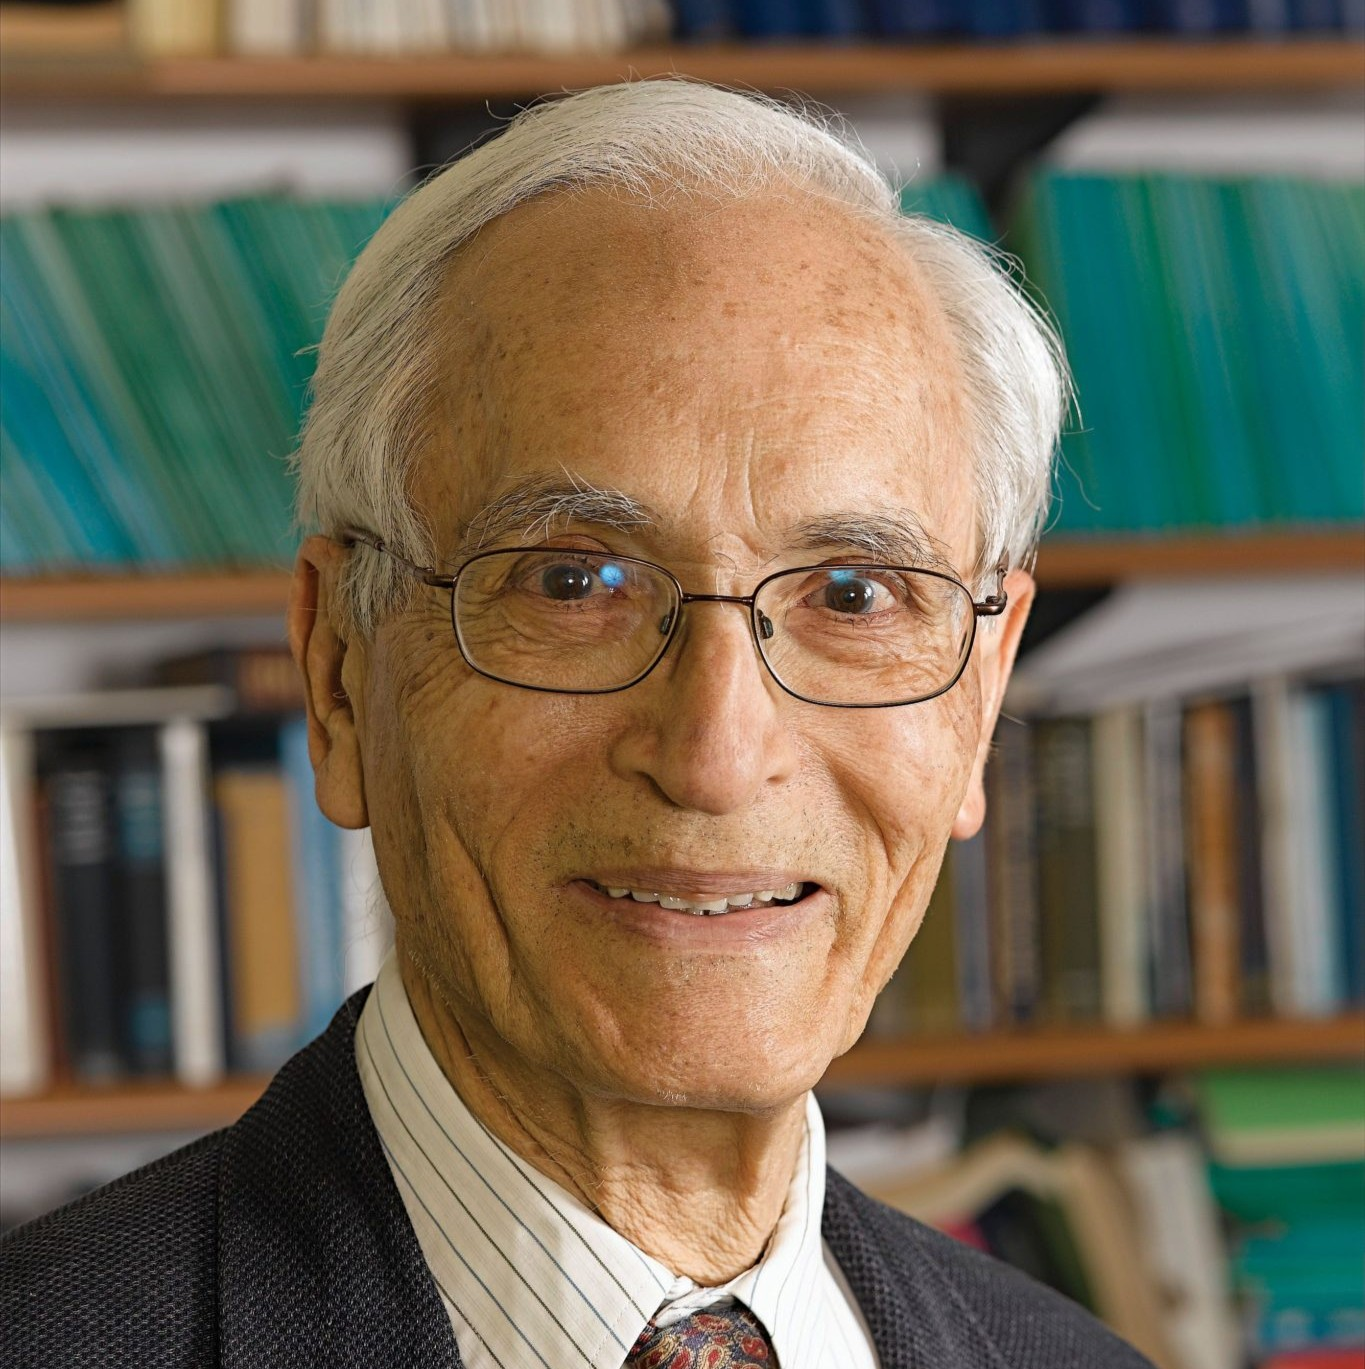
\includegraphics[width=\textwidth]{Figures/Ziv.jpeg}
%         \caption{Jacob Ziv}
%         \label{fig:ziv}
%     \end{subfigure}
    
%     \hfill
    
%     % 3rd image
%     \begin{subfigure}[b]{0.4\textwidth}
%         \centering
%         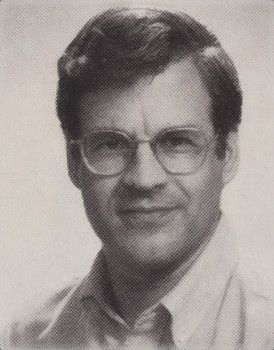
\includegraphics[width=\textwidth]{Figures/welch.jpg}
%         \caption{Terry Welch}
%         \label{fig:welch}
%     \end{subfigure}
%     \caption{Lempel - Ziv - Welch}
%     \label{fig:lzw}
% \end{figure}

% \begin{figure}[ht]
%  \centering
%  \begin{minipage}[b]{0.4\textwidth}
%   \centering
%   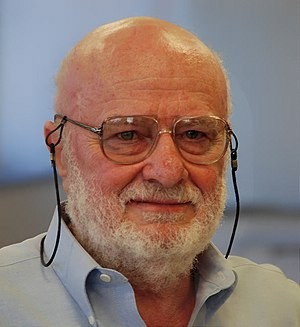
\includegraphics[height=0.85\textwidth]{Figures/lempel.jpg}
%   \caption{Abraham Lempel}
%  \end{minipage}%
%  \hfill
%  \begin{minipage}[b]{0.4\textwidth}
%   \centering
%   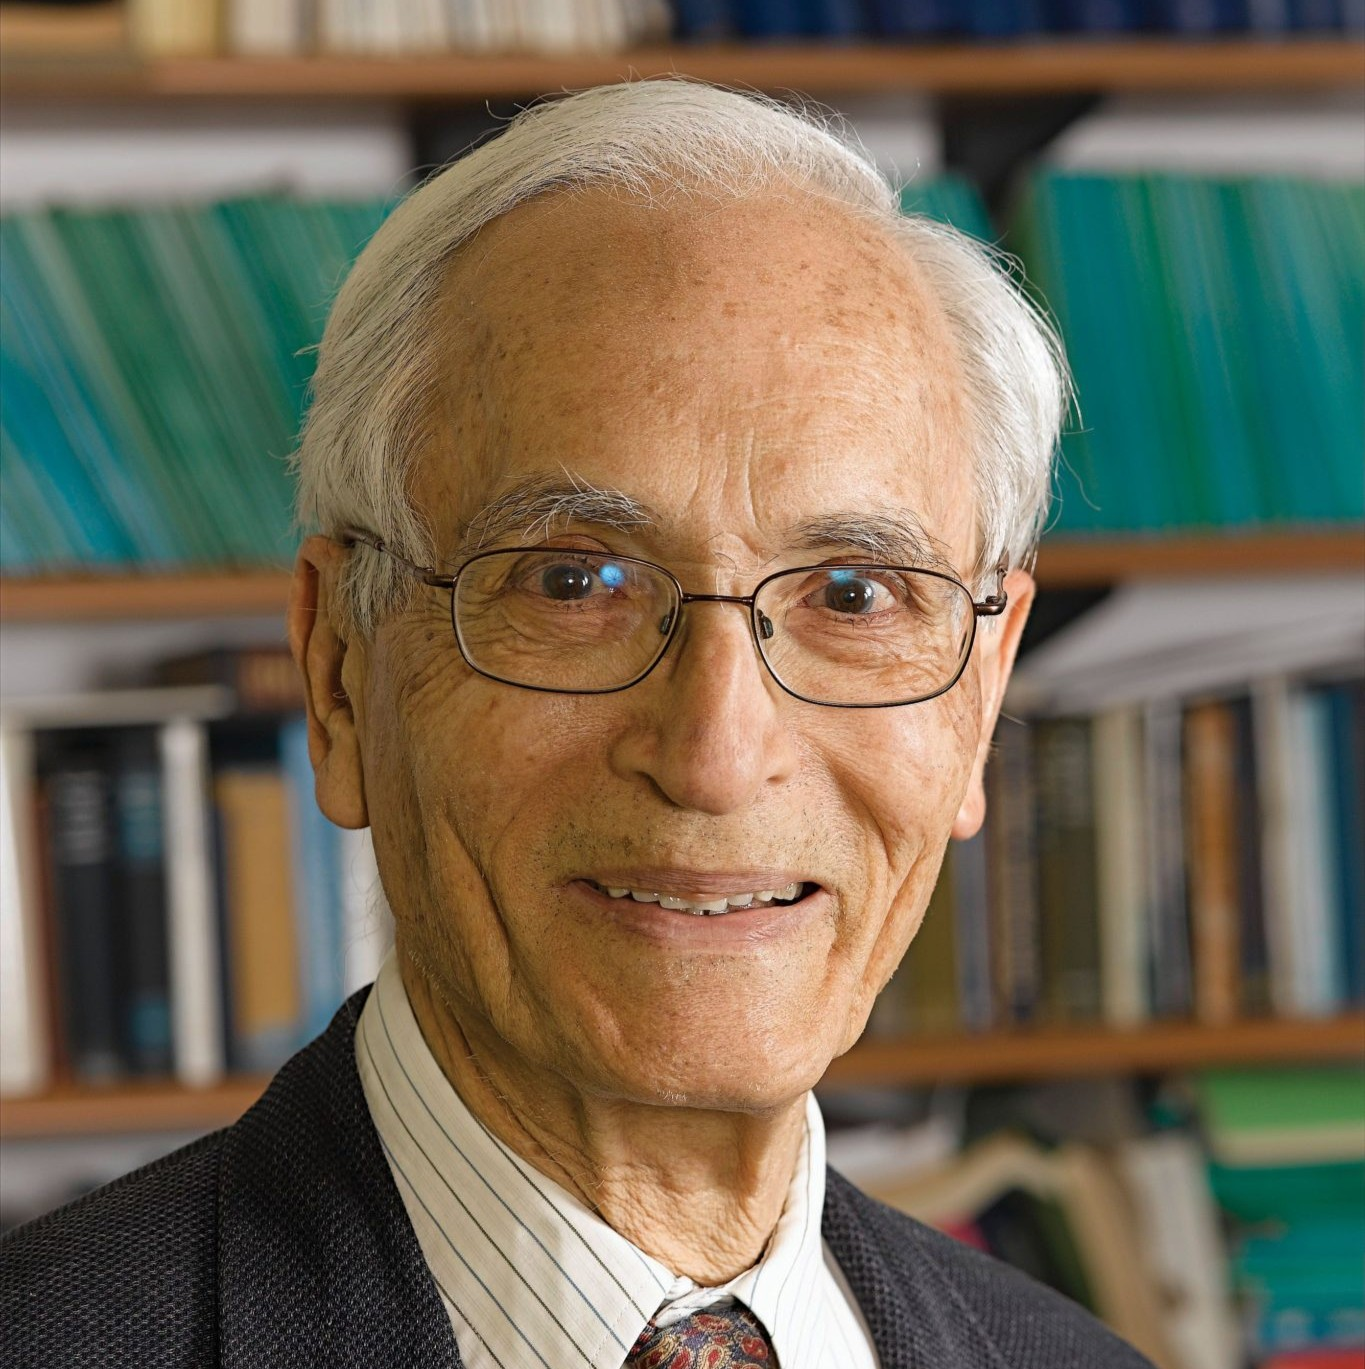
\includegraphics[height=0.85\textwidth]{Figures/Ziv.jpeg}
%   \caption{Jacob Ziv}
%  \end{minipage}

% \vskip\baselineskip
 
%  \begin{minipage}[b]{0.4\textwidth}
%   \centering
%   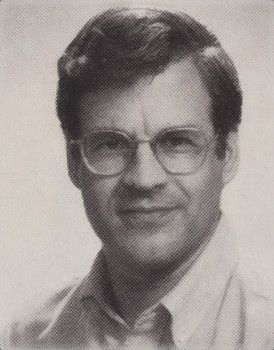
\includegraphics[height=0.85\textwidth]{Figures/welch.jpg}
%   \caption{Terry Welch}
%  \end{minipage}
% \end{figure}

\begin{figure}[ht]
    \centering
    \begin{minipage}{0.3\textwidth}
        \centering
        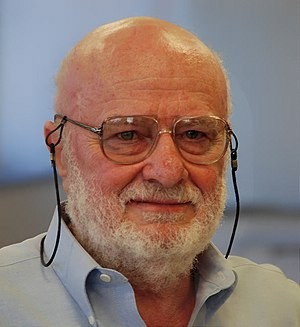
\includegraphics[width = \textwidth, height=1.1\textwidth]{Figures/lempel.jpg}
        \captionsetup{font=small}
        \caption{Abraham Lempel}
        \label{fig:fig1}
    \end{minipage}%
    \hfill
    \begin{minipage}{0.3\textwidth}
        \centering
        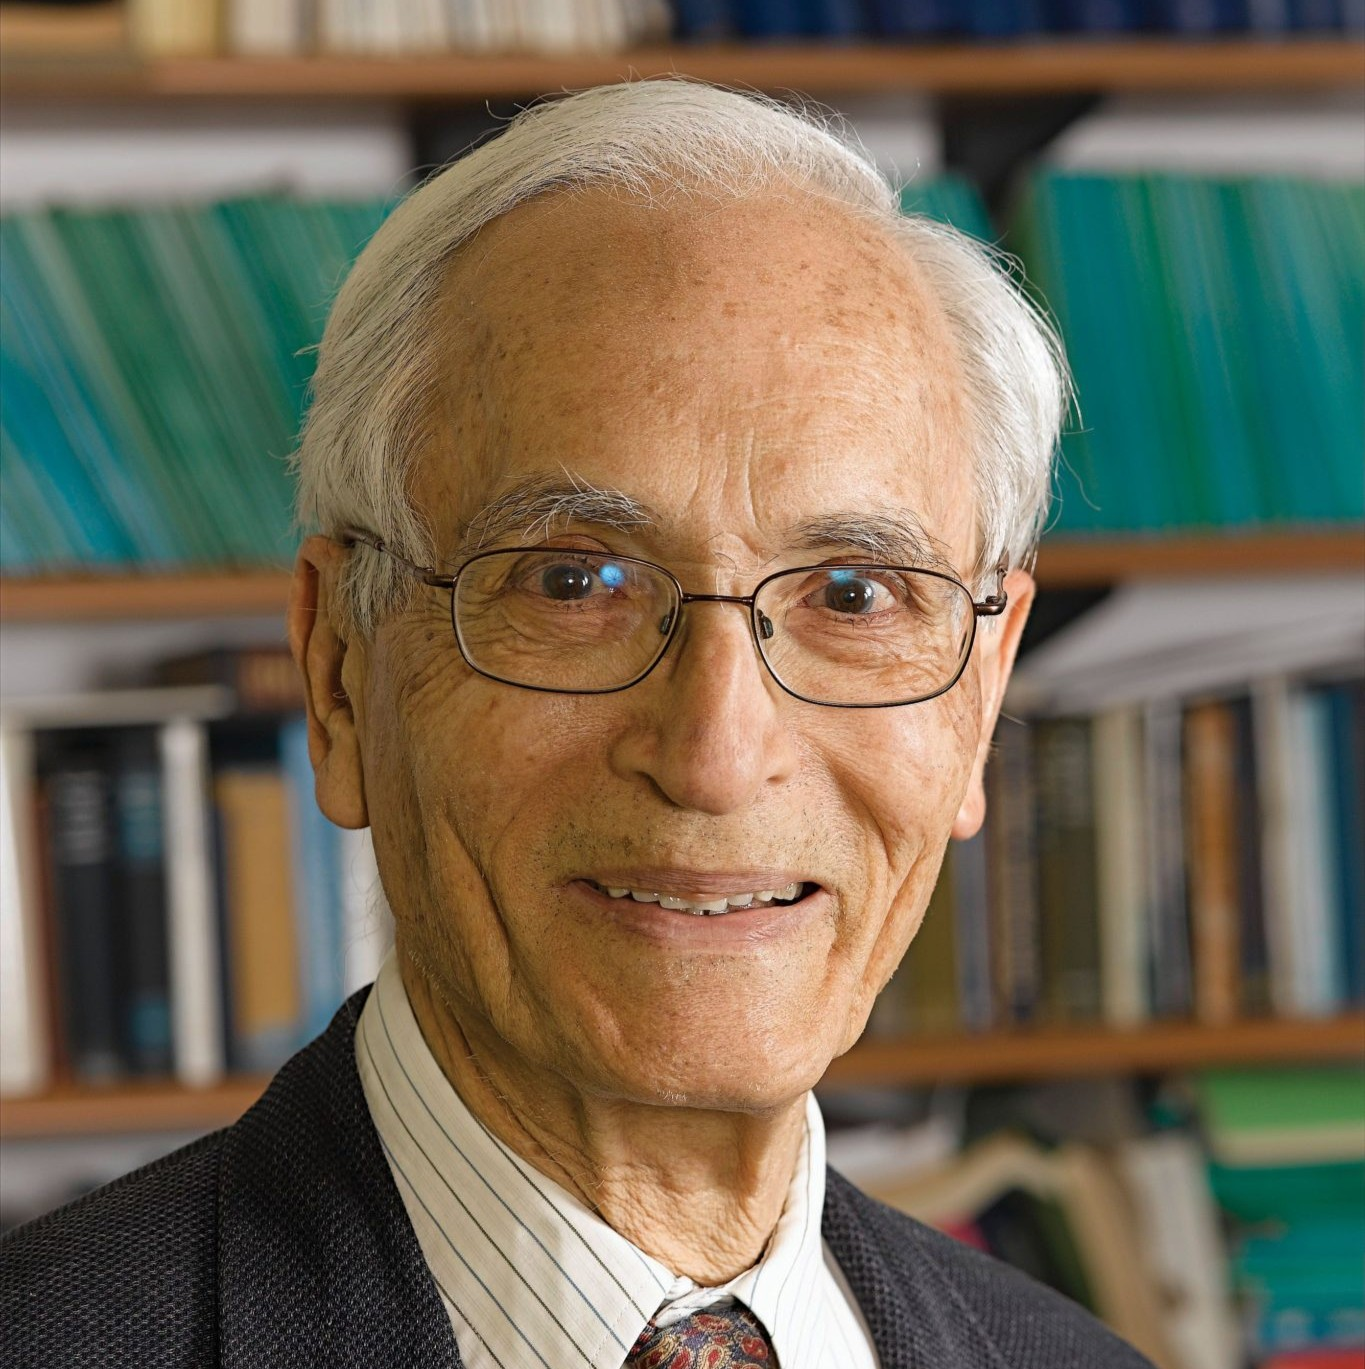
\includegraphics[width=\linewidth, height=1.1\textwidth]{Figures/Ziv.jpeg}
        \captionsetup{font=small}
        \caption{Jacob Ziv}
        \label{fig:fig2}
    \end{minipage}%
    \hfill
    \begin{minipage}{0.3\textwidth}
        \centering
        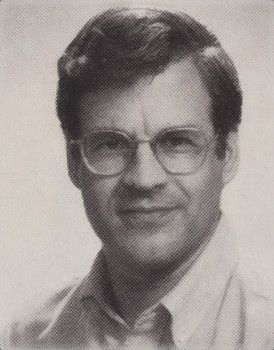
\includegraphics[width=\linewidth, height=1.1\textwidth]{Figures/welch.jpg}
        \captionsetup{font=small}
        \caption{Terry Welch}
        \label{fig:fig3}
    \end{minipage}
\end{figure}


The development of LZW arose from the need for efficient data compression methods during a time of rapidly growing digital information. Its design aimed to address the limitations of earlier compression methods by introducing a dynamic dictionary-based approach that did not require pre-analysis of the data. This adaptability marked a significant evolution in lossless compression techniques.

\vspace{10pt}

Unlike its predecessor LZ78, LZW uses a simplified mechanism to build and maintain its dictionary. This innovation made the algorithm computationally efficient and highly adaptable to various input data types, while preserving the core properties of the Lempel-Ziv methods. LZW's simplicity in logic allowed it to achieve high compression ratios without the complexity of earlier methods, making it a cornerstone in the history of data compression.